\documentclass[12pt]{article}
\usepackage{graphicx}
\usepackage{booktabs}
\usepackage[font=footnotesize,skip=5pt]{caption}
\usepackage[font=scriptsize,skip=0pt]{subcaption}
\usepackage{amsmath}
\usepackage{amsfonts}
\usepackage{amssymb}
\usepackage{lscape}
\usepackage{psfrag}
\usepackage[usenames]{color}
\usepackage{bbm}
\usepackage[update]{epstopdf}
\usepackage[bookmarks,pdfstartview=FitH,a4paper,pdfborder={0 0 0}]{hyperref}
\usepackage{verbatim}
\usepackage{listings}
\usepackage{textcomp}
\usepackage{course}
\usepackage{fancyhdr}
\usepackage{multirow}
\pagestyle{fancy}
\usepackage{tikz}
\usepackage{bm}
\usepackage{float}
%\usepackage{subfig}

\renewcommand{\sectionmark}[1]{\markboth{#1}{#1}}
\renewcommand{\subsectionmark}[1]{\markright{#1}}

\newtheorem{theorem}{Theorem}
\DeclareMathOperator{\Var}{Var}
\DeclareMathOperator{\Bias}{Bias}

\graphicspath{ {Images/} }
\usepackage[backend=biber, style=bwl-FU, sorting=nyt]{biblatex}
\addbibresource{bib.bib}

\fancyhf{}
\fancyhead[RO]{\nouppercase{\footnotesize\sc\leftmark\ \hrulefill\ \thepage}}
%\fancyhead[RE]{\nouppercase{\footnotesize\sc\thepage\ \hrulefill\ }}
\renewcommand{\headrulewidth}{0pt}

\makeatletter
\def\cleardoublepage{\clearpage\if@twoside \ifodd\c@page\else%
\hbox{}%
\thispagestyle{empty}%
\clearpage%
\if@twocolumn\hbox{}\clearpage\fi\fi\fi}
\makeatother


\renewcommand{\topfraction}{0.9}  % max fraction of floats at top
\renewcommand{\bottomfraction}{0.8} % max fraction of floats at bottom
% Parameters for TEXT pages (not float pages):
\setcounter{topnumber}{2}
\setcounter{bottomnumber}{2}
\setcounter{totalnumber}{4}            % 2 may work better
\setcounter{dbltopnumber}{2}           % for 2-column pages
\renewcommand{\dbltopfraction}{0.9}    % fit big float above 2-col. text
\renewcommand{\textfraction}{0.07}     % allow minimal text w. figs
% Parameters for FLOAT pages (not text pages):
\renewcommand{\floatpagefraction}{0.7}  % require fuller float pages
% N.B.: floatpagefraction MUST be less than topfraction !!
\renewcommand{\dblfloatpagefraction}{0.7} % require fuller float pages

\sloppy

\widowpenalty=10000
\clubpenalty=10000

\edef\today{%\number\day\
\ifcase\month\or
January\or February\or March\or April\or May\or June\or July\or
August\or September\or October\or November\or December\fi\ \number\year}
\title{\vspace*{40.0mm}
  \bf Report on project about principal component analysis
         \vspace*{20.0mm} \\
  %\vspace{-20mm}\framebox{DRAFT VERSION}\vspace{20mm} \\
  \Large\bf Statistical Data Analysis 
  
 
  
  Project 1 \vspace*{20.0mm}
  \vspace*{40.0mm}}
\author{Mitja Mandić}
\date{ April 2022}

\begin{document}

\begin{figure}
  \parbox[t]{125mm}{
    \vspace*{6mm}
    \scriptsize\sf           DEPARTMENT OF MATHEMATICS \\
    \scriptsize\sf           FACULTY OF SCIENCE\\
    \scriptsize\sf           KU LEUVEN}
  \parbox[t]{40mm}{
    \begin{flushright}
      
\includegraphics[height=15mm]{../images/logo.eps.pdf}
    \end{flushright}}
\end{figure}

\maketitle
\thispagestyle{empty}
\raggedbottom

\cleardoublepage
\pagenumbering{roman}
\setcounter{tocdepth}{2}
%\tableofcontents
\pagenumbering{arabic}

\section{Introduction}
For the first project we are analysing the spectroscopy dataset of four different types of cantaloupe melons. Each spectra was measured on 256 wavelengths of 2158 melons.
In \label{fig:spectra} we plot the spectra of the whole dataset.
\begin{figure}[h!]
    \begin{subfigure}[b]{0.5\linewidth}
        \centering
        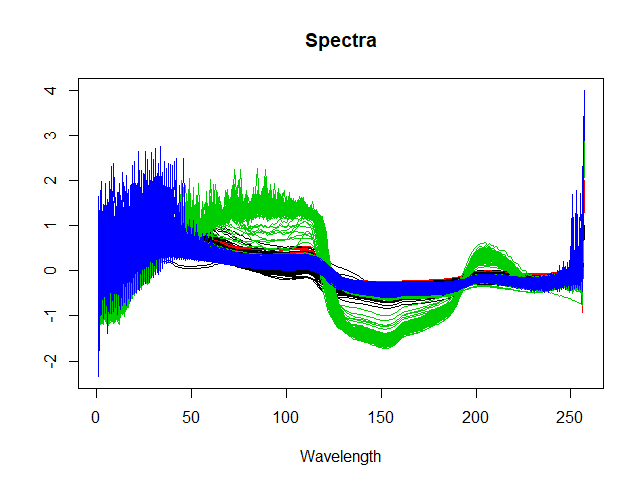
\includegraphics[width=\textwidth]{../images/spectra.png}
     \caption{Spectral plot of the whole dataset}\label{fig:spectra}
    \end{subfigure}%
    %
    \begin{subfigure}[b]{0.5\linewidth}
        \centering
     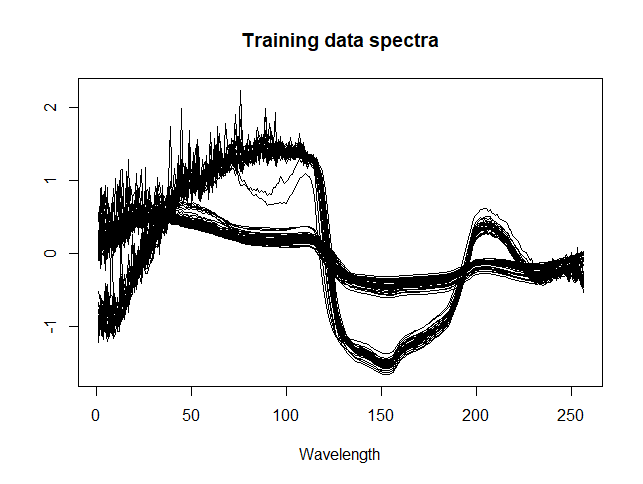
\includegraphics[width=\textwidth]{../images/trainDataSpectra.png}
     \caption{Spectral plot of the training data}\label{fig:trainDataSpectra}
    \end{subfigure}%
   \caption{Spectral plots of both the whole and training data datasets}
\end{figure}
Apart from the cultivar ``Ha'' we seem to have a rather homogenous dataset, where most of variance seem to be happening in the first 50 variables. In the ``Ha'' group this 
extends to around 200 variables.

Out of the main dataset we randomly select 180 (90 for training and 90 for test data) cantaloupes -- in our case,
rather interestingly, this whole sample consists only of members of group ``Ha''. 

\section{Classical PCA} \label{classicPCA}
We perform classical PCA on a part of the original dataset. Before we continue, we check for differences between variances of the variables.

As we can see in figure \ref{fig:var}, there are some variables with much higher variance than others. That is why we will base our further PCA analysis on correlation matrix rather than
covariance matrix. Next to it in figure \ref{fig:scree} a scree plot is shown - based on that we decide to keep two variables, as they explain over 90\% total variance.

\begin{figure}[h!]
    \begin{subfigure}[b]{0.5\linewidth}
        \centering
        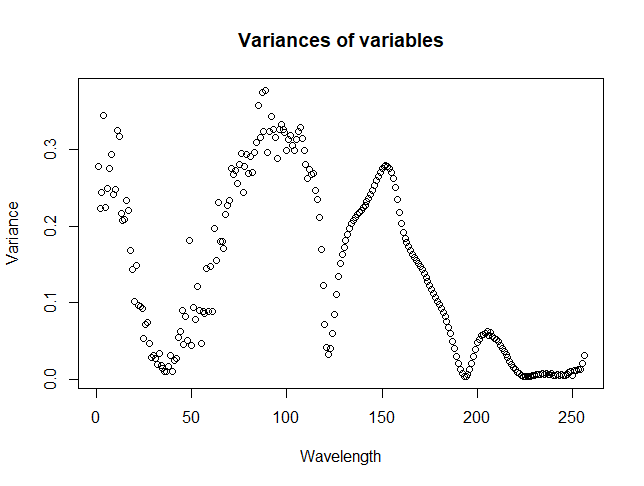
\includegraphics[width=\textwidth]{../images/variances.png}
     \caption{Variances of each component vary in size}\label{fig:var}
    \end{subfigure}%
    %
    \begin{subfigure}[b]{0.5\linewidth}
        \centering
     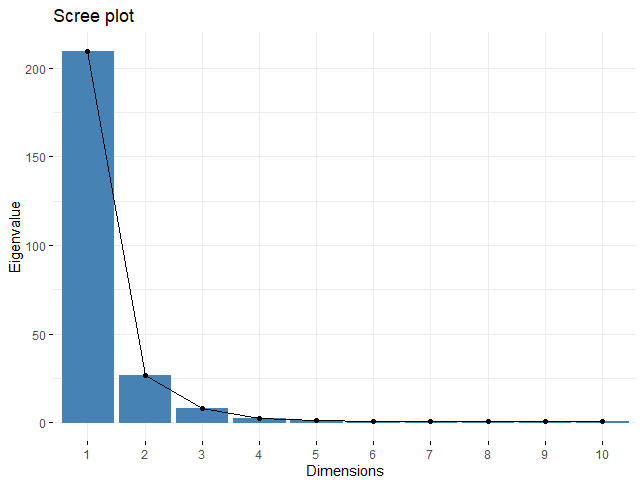
\includegraphics[width=\textwidth]{../images/screePlot.png}
     \caption{Scree plot, showing eigengvalues in descending order - first two are much larger than the rest}\label{fig:scree}
    \end{subfigure}%
   \caption{Figures of variances and scree plot}
\end{figure}

Classic PCA of training data based on two components flags five points as outliers (surpassing the score and/or orthogonal distance cutoff) - these are cantaloupes 
number 14,33,42,48 and 88. In the outlier plot depicted on \ref{fig:outlierClassic} we notice formation of two groups, which is confirmed when we plot the scores, which
we then see on figure \ref{fig:scoresClassic}.

\begin{figure}[h!]
  \begin{subfigure}[b]{0.5\linewidth}
      \centering
      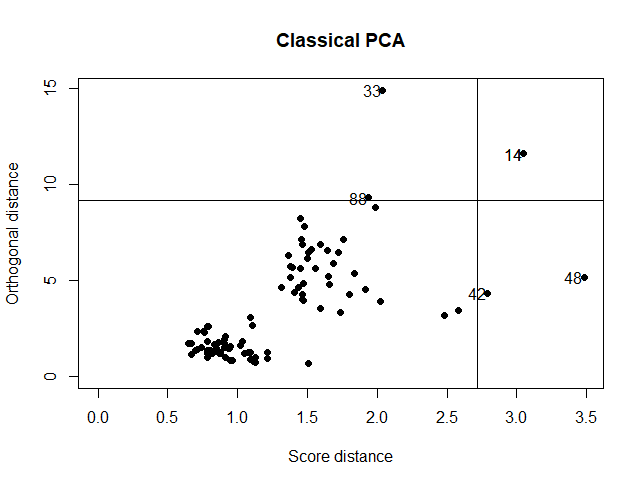
\includegraphics[width=\textwidth]{../images/outliersClassic.png}
   \caption{Outlier plot of PCA based on 2 components}\label{fig:outlierClassic}
  \end{subfigure}%
  %
  \begin{subfigure}[b]{0.5\linewidth}
      \centering
   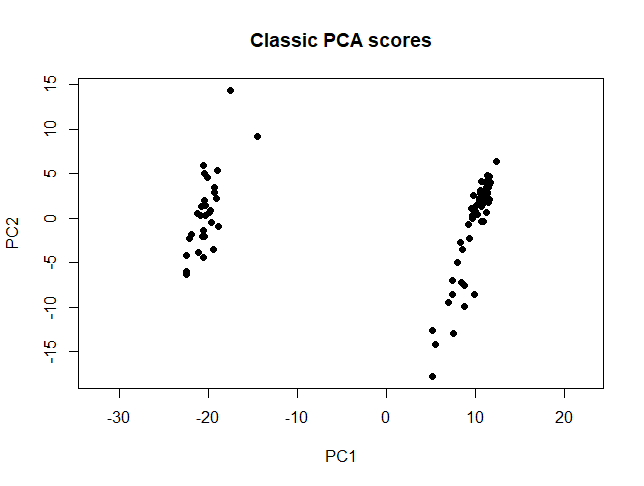
\includegraphics[width=\textwidth]{../images/ClassicPCAScores.png}
   \caption{Scores of classic PCA}\label{fig:scoresClassic}
  \end{subfigure}%
 \caption{Outlier plot and scores of classic PCA.}
\end{figure}

\section{Robust PCA}
In this section we comment on results obtaining by performing robust principal component analysis of the training data. For this we use function \texttt{PcaHubert} from the
package \texttt{rrcov}, with scale parameter set to \texttt{mad.} Interestingly, we obtain quite different results compared to classical PCA analysis. To facilitate
the discussion, we recreate the plots seen in section \ref{classicPCA}.

\begin{figure}[h!]
  \begin{subfigure}[b]{0.5\linewidth}
      \centering
      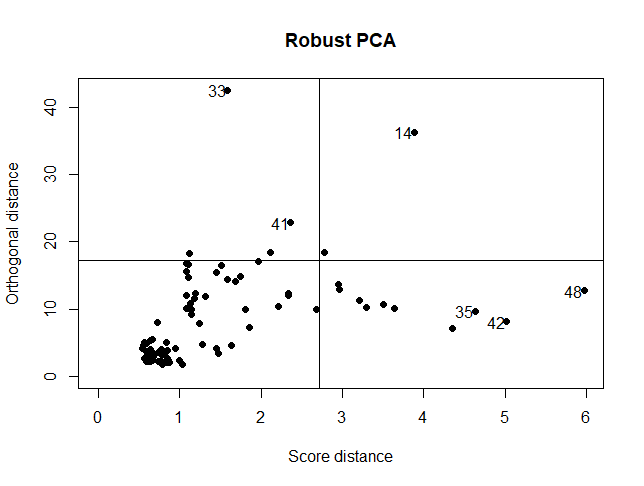
\includegraphics[width=\textwidth]{../images/robustPCAoutliers.png}
   \caption{Outlier plot of PCA based on 2 components}\label{fig:robustOutliers}
  \end{subfigure}%
  %
  \begin{subfigure}[b]{0.5\linewidth}
      \centering
   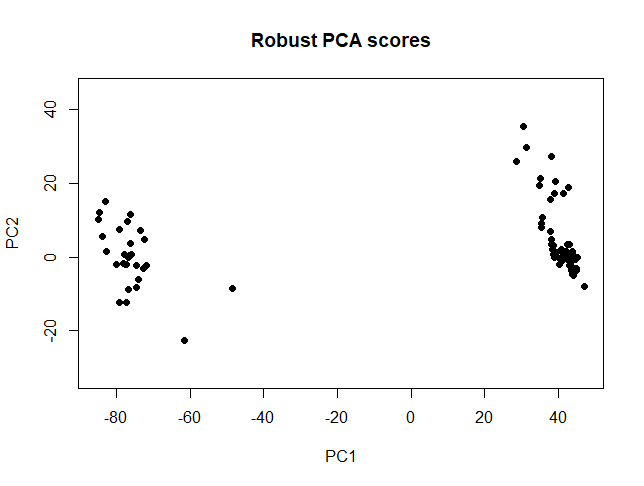
\includegraphics[width=\textwidth]{../images/robustPCAscores.png}
   \caption{Scores of robust PCA}\label{fig:scoresRobust}
  \end{subfigure}%
 \caption{Outlier plot and scores of robust PCA.}
\end{figure} 

Firtly we notice that much more points are exceeding the score or orthogonal distance cutoff. 
Additionally, one more point has both orthogonal and score distance larger than cutoffs than in the classical case (point 14). Outliers detected by this method
are also much further from the main data cloud than those detected in previous section.

Another thing we notice comparing figures \ref{fig:scoresRobust} and \ref{fig:scoresClassic} is that in the former case the two groups are much further apart. Let us
now try to find the origin of such behaviour. In \ref{fig:trainDataSpectra} we see that two groups seem to differ at, for example, 100th wavelength, with one group having
values around 0 and the other between 1 and 2. After separating them like this, we see that this are the groups also found by PCA, as seen in \ref{twoGroupScore}.

\begin{figure}
  \begin{center}
    \centering
      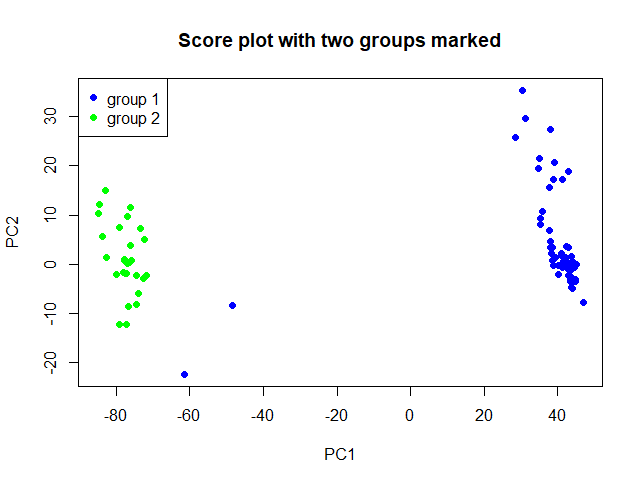
\includegraphics[width=0.5\textwidth]{../images/twoGroupScore.png}
      \caption{Score plot obtained by robust PCA with two groups marked}
      \label{fig:twoGroupScore}
  \end{center}
\end{figure}

Because of such differences between the two methods and rather unusal data, we decide to proceed to further questions with robust PCA.

\section{Validation set analysis}
Now we take a look at the other half of data set we selected in the beginning. We compute scores and
predicted values of the validation set with respect to the values obtained by performing robust PCA on training data.

Outlier plot, containing values from training data and calculated validation data scores is presented in figure \ref{fig:outlierPred}.
\begin{figure}[h!]
  \begin{center}
    \centering
    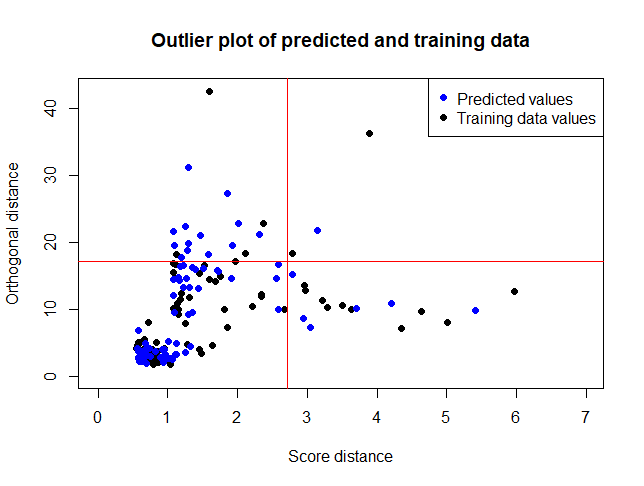
\includegraphics[width=0.5\textwidth]{../images/outlierPred.png}
    \caption{Outlier plot of training and predicted data}
    \label{fig:outlierPred}
  \end{center}
\end{figure}

We see that dataclouds in the bottom left aling rather nicely. On the other hands, outliers are more dispersed when 
considering predicted data, especially in the orthogonal distance. We assume that the second data cloud of predicted values might 
be affected by the two severe orthogonal outliers found in robust PCA (points 14 and 33). 

Similar amount of outliers are found in score distance.

Plotting the spectra of predicted and actual data gives satisfying results, with plots looking very similar.
\begin{figure}[h!]
  \begin{subfigure}[b]{0.5\linewidth}
      \centering
      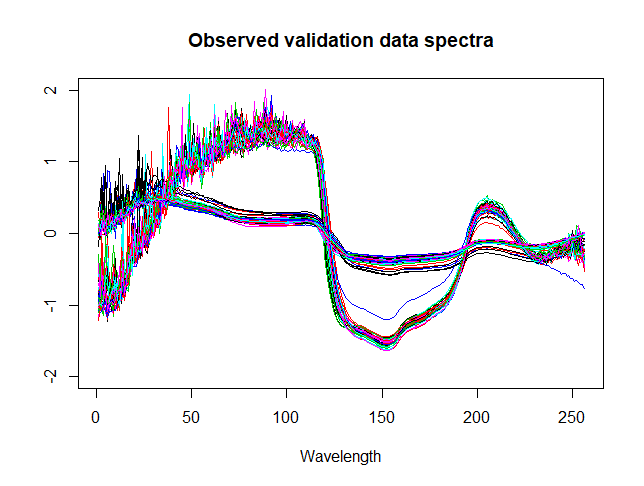
\includegraphics[width=\textwidth]{../images/validDataSpectra.png}
   \caption{Spectral plot of the validation data}\label{fig:validDataSpectra}
  \end{subfigure}%
  %
  \begin{subfigure}[b]{0.5\linewidth}
      \centering
   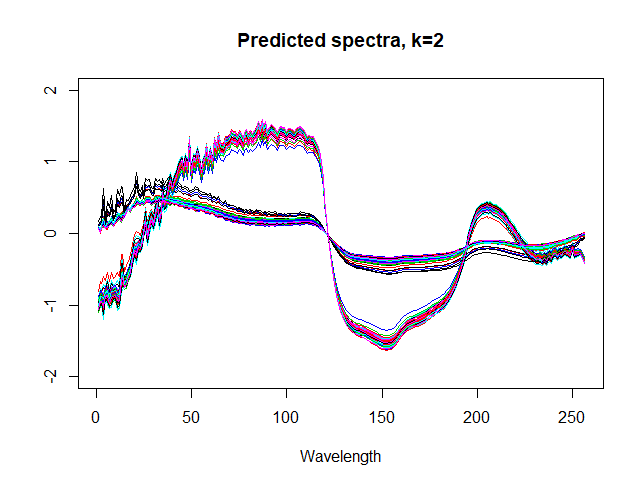
\includegraphics[width=\textwidth]{../images/predictedSpectra.png}
   \caption{Predicted spectral plot}\label{fig:predictedSpectra}
  \end{subfigure}%
 \caption{Figures comparing predicted and observed spectra.}
\end{figure}

\section{Normality of training data}
In the final section of the report we investigate whether the clean training dataset can be assumed to be sampled from a normal distrbution.
We take into accound outliers found by robust PCA, that is points exceeding orthogonal and/or score distance cutoff. 

There are 16 such points found, which we then remove from the dataset. Shapiro-Wilk test strongly rejects normality with p-value 
$1.768\cdot 10^{-12}.$ Plotting the regular and removed values we can see that there still are two groups present, which makes it
easier to understand such a low p-value.
\begin{figure}[ht!]
  \begin{center}
    \centering
      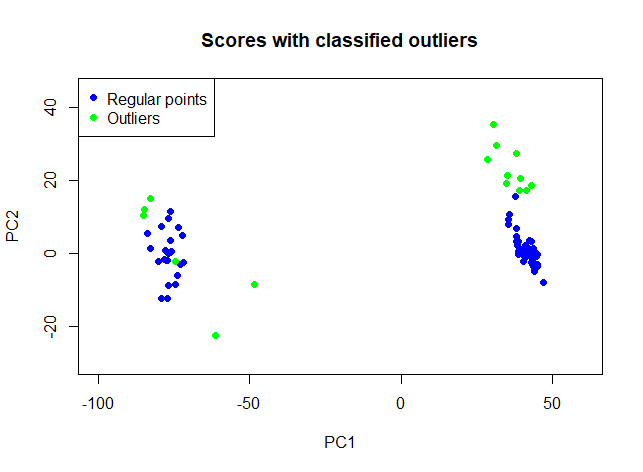
\includegraphics[width=0.5\textwidth]{../images/regularAndOutliers.png}
      \caption{Plot of scores of regular and outlying points.}
      \label{fig:regularAndOutliers}
  \end{center}
\end{figure}

Scores in this case certainly are not unimodally normally distributed, as we have found two very clear groups. However, we might consider investigating normality of scores of
each group separately.


\end{document}
